\title{WiMAX Measurements \\
{\small CS707 Assignment 1}
}
\author{
    Robert Jellinek, Siva Ramasubramanian \\
    University of Wisconsin-Madison \\
    \{jellinek, sivas\}@cs.wisc.edu
}
\date{\today}

\documentclass[12pt]{article}
\usepackage[hyphens]{url}
\usepackage[margin=1.5in]{geometry}
\usepackage{graphics,epsfig}
\newcommand{\fixme}[1]{\textcolor{red}{[FIXME: #1]}}

\begin{document}
\maketitle

%\begin{abstract}
%\end{abstract}

\section{Introduction}
For this project, our goal was to take 20 measurements---10 line-of-sight (LOS)
and 10 non-line-of-sight (NLOS)---of statistics describing the quality of the
channel between the WiMAX station at the top of the Computer Sciences building.
Our goal was to record a set of measurements that was diverse enough to use to
build a model that takes a set of GPS coordinates as parameters and returns the
predicted signal strength. That is, we hypothesize that our signal-strength
measurements, when used under an appropriate model, can predict signal strength
at other locations.

\section{Methodology} We collected our measurements by walking from point to
point, arranging the WiMAX dongle such that it faced the access point (AP)
antenna on the top of the Computer Sciences building, and running a number of
tests five times each at each location. We made sure that we did not stand
between our WiMAX antenna and the AP in order to avoid interfering with (i.e.
weakening) the signal.  We used the WiMAX card's web-based management interface
tool to collect data on RSSI and CINR. We then used \textit{iperf} to record
data on the card's uplink speed, and \textit{speedtest.net} to measure the
link's downlink speed. We also recorded time, and used the Locus app on an
Android phone to record and plot the GPS coordinates of our measurements.

Our LOS data was captured by walking up Monroe St., making sure the WiMAX
antenna was visible from our position, and performing the tests mentioned above.
For our NLOS tests, we walked some distance from Monroe St. such that our
position obscured our view of the WiMAX antenna. While we attempted to diversify
our range of locations, dusk and impending rain forced us to remain close to
Monroe St. The final two LOS and final three NLOS data points were recorded one
day after the other measurements. Measurements are visible in Figure
\ref{fig:locations}.

%% TODO include location plots here
\begin{figure}[t]
\center
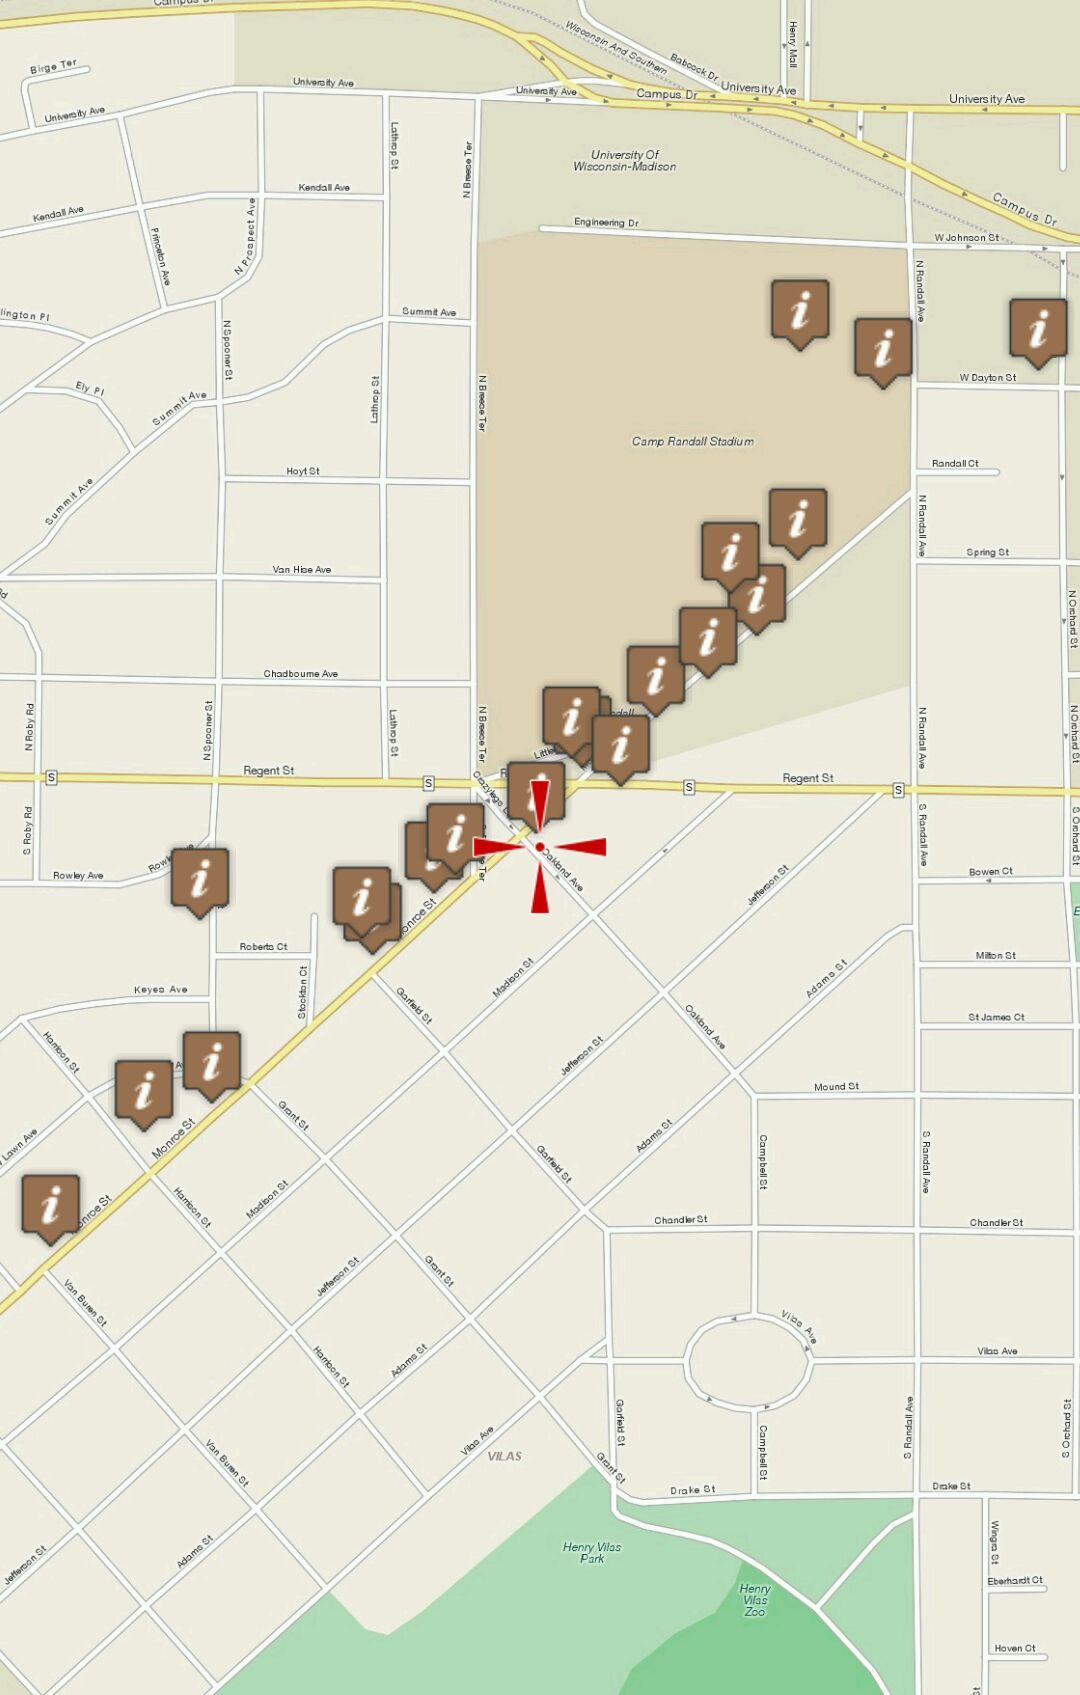
\includegraphics[width=.5\linewidth]{locations}
\caption{Locations of our LOS and NLOS measurements.}
\label{fig:locations}
\end{figure}

\section{Model} 
Our model depends on handling LOS and NLOS measurements separately, since even
though two sampling locations can be geographically very close, the introduction
of obstacles in the signal path can have a substantial effect on signal
strength. The goal of each model is to predict RSSI and downlink throughput as a
function of GPS coordinates. We discuss each case in turn.

\subsection{LOS Model} We approached the LOS model as follows. At each of 10
locations, we collected 5 LOS tests and average them. For each distance from the
AP $d_{1}~..~d_{10}$, we used the \textit{polyfit} linear regression function in
Matlab to predict the corresponding RSSIs $r_{1}~..~r_{10}$.
Similarly, each of the 10 distances $d_{i}$ there is a corresponding downlink
value $s_{i}$ measured using \textit{speedtest.net}.  Similarly, we used
Matlab's \textit{polyfit} function to model downlink speed as a function of
the receiver's distance from the AP, such that $r_{i} \cdot s_{i} = f(d_{i}$ for
each set of measurements $i$. 
\fixme{We should say more about why we used polyfit for both of these, and
possibly something about why it's better than other methods. Also, what does
polyfit take as parameters? GPS coords? Just distances as scalars? And what are
the results? Also, were the inputs to this model the individual measurements,
or just the average from each location? -Rob} 

\subsection{NLOS Model}
\fixme{TODO}

\section{Results and Conclusion}
\fixme{TODO: what were our results?}
Though we have not yet had the opportunity to test our model on data points
besides our own, we believe that it will be mostly accurate in its predictions,
particularly in the case of the LOS measurements, where we hypothesize that
distance will be a more heavily weighted factor in predicting RSSI and downlink
speed.
For NLOS measurements, on the other hand, we hypothesize that distance---the
sole input to our models, as calculated from the GPS coordinates of our
measurements---is a relatively weaker predictor of signals strength. In
particular, we suspect that the nature of the obstacle in the signal path of our
NLOS measurements will play a larger role in the attenuation of the signal than
will distance, and so should probably be an input to any model of signal
strength. Unfortunately, characterizing the nature of particular obstacles
between two arbitrary points in a city seems to be a non-trivial task, and so
the most effective approach is likely to be the one that combines samples from
as many locations as possible in the target location, and simply averages the
measurements of the locations nearest to the point of interest.

%\bibliographystyle{abbrv}
%\bibliography{biblio}

\end{document}
